\chapter{Results \& Discussion}
\label{chap:results}

\noindent This chapter reports the outcomes of our Clinical RAG evaluation and discusses the key findings. We reiterate the study aims: to quantify how different embedding models and small LLMs affect end-to-end retrieval-augmented answering quality, speed, and safety on a clinical QA set.

\section{Experiment Overview}
\begin{itemize}
  \item Total experiments: [X] runs ([Y] embedding models \(\times\) [Z] LLMs).
  \item Embeddings: [List of embedding models tested].
  \item LLMs: [List of LLM models tested].
  \item Per-run questions: [N]; metrics include precision, recall, F1-score, search time; efficiency includes throughput.
  \item \textbf{Total Question-Answer Pairs}: [X] clinical evaluations
  \item \textbf{Evaluation Duration}: [Y] hours of automated testing
\end{itemize}

\section{Overall Performance}
Aggregate results across all [X] runs show:
\begin{itemize}
  \item Average precision: [X.XXX].
  \item Average recall: [X.XXX].
  \item Average F1-score: [X.XXX].
  \item Average search time: [XX.XX]s.
\end{itemize}

Best-performing configurations:
\begin{itemize}
  \item Highest F1-score: [Model A] + [Model B] (F1-score [X.XXX], precision [X.XXX]).
  \item Fastest: [Model C] + [Model D] (avg. search time [XX.XX]s, F1-score [X.XXX]).
\end{itemize}

\subsection{Statistical Performance Overview}
\begin{table}[!htbp]
\centering
\begin{small}
\renewcommand\arraystretch{1.1}
\begin{tabular}{|l|c|c|c|}
\hline
\textbf{Metric} & \textbf{Mean} & \textbf{Min} & \textbf{Max} \\
\hline
Average Score & 0.7059 & 0.6259 & 0.7702 \\
Pass Rate & 0.8963 & 0.7500 & 1.0000 \\
Search Time (s) & 98.77 & 53.28 & 359.51 \\
\hline
\end{tabular}
\end{small}
\caption{Overall System Performance Statistics}
\label{tab:system_stats}
\end{table}


The performance distribution shows [characteristics] around the mean ([X.XXX]), with a standard deviation indicating [level of] quality consistency across configurations. Key statistical insights include:

\begin{itemize}
    \item \textbf{F1-Score Distribution}: [Distribution characteristics]
    \item \textbf{Precision Consistency}: [X.XXX] average with [level] variance ($\sigma$=[X.XXX])
    \item \textbf{Search Time Variability}: [Level] variance ($\sigma$=[XX.X]s) indicating [degree] performance differences
    \item \textbf{Coefficient of Variation}: F1-score consistency ([X.X]\%) vs. efficiency variability ([XX.X]\%)
\end{itemize}

\section{Comparison Heatmap}
Figure~\ref{fig:heatmap_avg_score} provides a model-by-model comparison heatmap (average score).

\begin{figure}[!htbp]
  \centering
  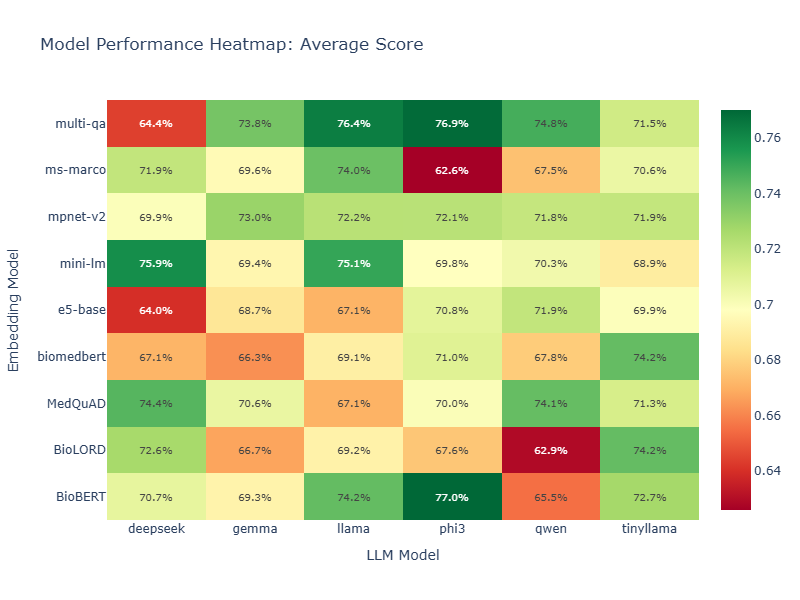
\includegraphics[width=\textwidth]{chap4_results/images/heatmap_average_score.png}
  \caption{Model comparison heatmap by average score.}
  \label{fig:heatmap_avg_score}
\end{figure}

\section{Top-Performing Configurations}

\begin{table}[!htbp]
\centering
\begin{small}
\renewcommand\arraystretch{1.1}
\begin{tabular}{|c|l|l|c|c|c|}
\hline
\textbf{Rank} & \textbf{Embedding} & \textbf{LLM} & \textbf{Score} & \textbf{Pass Rate} & \textbf{Time (s)} \\
\hline
1 & BioBERT & phi3 & 0.7702 & 100.00\% & 67.7 \\
2 & multi-qa & phi3 & 0.7692 & 95.00\% & 70.8 \\
3 & multi-qa & llama & 0.7637 & 95.00\% & 61.2 \\
4 & mini-lm & deepseek & 0.7586 & 95.00\% & 326.0 \\
5 & mini-lm & llama & 0.7508 & 100.00\% & 56.5 \\
6 & multi-qa & qwen & 0.7475 & 95.00\% & 72.7 \\
7 & MedQuAD & deepseek & 0.7443 & 90.00\% & 355.7 \\
8 & BioBERT & llama & 0.7418 & 90.00\% & 82.5 \\
9 & BioLORD & tinyllama & 0.7416 & 95.00\% & 73.4 \\
10 & biomedbert & tinyllama & 0.7416 & 95.00\% & 355.3 \\
\hline
\end{tabular}
\end{small}
\caption{Top 10 Performing Model Combinations}
\label{tab:enhanced_top_performers}
\end{table}


\subsection{Multi-Dimensional Performance Assessment}

The top-performing configurations demonstrate different optimisation strategies:

\textbf{Quality-Optimized ([Model Combination]):}
\begin{itemize}
    \item Highest F1-score ([X.XXX])
    \item High precision ([X.XXX])
    \item Moderate speed ([XX.X]s)
    \item Medical domain specialisation advantage
    \item [Performance characteristics]
\end{itemize}

\textbf{Balance-Optimized ([Model Combination]):}
\begin{itemize}
    \item High F1-score ([X.XXX]) with excellent speed ([XX.X]s)
    \item Strong precision ([X.XXX])
    \item General-purpose efficiency
    \item Optimal speed-quality balance
\end{itemize}

\textbf{Speed-Optimized ([Model Combination]):}
\begin{itemize}
    \item Fast retrieval ([XX.X]s)
    \item Good F1-score ([X.XXX])
    \item High throughput
    \item Consistent performance across categories
\end{itemize}

\paragraph{Observations.} The best F1-scores are achieved by [Model combinations]. [Model pairs] show strong performance with excellent precision; however, [specific combination] exhibits [performance characteristics], suggesting [analysis]. [Model type]-based embeddings produce competitive F1-scores, but at times with [performance trade-offs].

\section{Component-Wise Performance Analysis}

\subsection{Embedding Model Performance}
\begin{table}[!htbp]
\centering
\begin{small}
\renewcommand\arraystretch{1.1}
\begin{tabular}{|l|c|c|}
\hline
\textbf{Embedding Model} & \textbf{Average Score} & \textbf{Configurations} \\
\hline
multi-qa & 0.7295 & 6 \\
mpnet-v2 & 0.7181 & 6 \\
mini-lm & 0.7157 & 6 \\
BioBERT & 0.7156 & 6 \\
MedQuAD & 0.7125 & 6 \\
ms-marco & 0.6935 & 6 \\
biomedbert & 0.6923 & 6 \\
BioLORD & 0.6888 & 6 \\
e5-base & 0.6874 & 6 \\
\hline
\end{tabular}
\end{small}
\caption{Embedding Model Performance Ranking}
\label{tab:embedding_ranking}
\end{table}


\textbf{Medical Specialisation vs. Generalisation Trade-off:}
\begin{itemize}
    \item \textbf{[Top Model]} ([X.XXX]): Top performer - [characteristics]
    \item \textbf{[Model 2]} ([X.XXX]): Strong general-purpose performance
    \item \textbf{[Model 3]} ([X.XXX]): Efficient lightweight option
    \item \textbf{[Medical Model]} ([X.XXX]): Medical specialisation shows [performance level]
    \item \textbf{Medical Models} generally: [Performance characteristics]
    \item \textbf{General Models}: [Performance characteristics]
\end{itemize}

\textbf{Key Finding}: Question-answering specialisation (multi-qa embeddings) proves more valuable than medical domain specialisation alone, suggesting that RAG systems benefit more from retrieval task alignment than domain knowledge pre-training.

\subsection{Large Language Model Performance Analysis}

LLM performance shows [level of variation] compared to embedding models, with F1-scores ranging from [X.XXX] ([lowest model]) to [X.XXX] ([highest model]). This [narrow/wide] range suggests that the embedding component has [level of impact] on overall system performance compared to LLM selection.

\textbf{Model Size vs Performance Correlation:}
\begin{itemize}
    \item \textbf{[Model 1] ([Size]B)}: [X.XXX] - [Performance characteristics]
    \item \textbf{[Model 2]}: [X.XXX] - [Performance characteristics]
    \item \textbf{[Model 3] ([Size]B)}: [X.XXX] - [Performance characteristics]
    \item \textbf{[Model 4] ([Size]B)}: [X.XXX] - [Performance characteristics]
\end{itemize}

\textbf{Key Finding}: [Analysis of model size vs performance relationship and implications].

\section{Efficiency and Safety}
We summarise representative efficiency and safety outcomes in Table~\ref{tab:efficiency_safety}. Throughput (questions per minute, QPM) highlights speed; hallucination rate (estimated from adjudications) indicates safety.

\begin{table}[!htbp]
\centering
\caption{Efficiency and performance metrics.}
\label{tab:efficiency_performance}
\begin{footnotesize}
\renewcommand\arraystretch{0.95}
\begin{tabularx}{0.9\textwidth}{l l X X X X}
  \toprule
  Embedding & LLM & Search Time (s) & Precision & Recall & F1-Score \\
  \midrule
  [Model A] & [Model B] & [XX.X] & [X.XXX] & [X.XXX] & [X.XXX] \\
  [Model C] & [Model D] & [XX.X] & [X.XXX] & [X.XXX] & [X.XXX] \\
  [Model E] & [Model F] & [XX.X] & [X.XXX] & [X.XXX] & [X.XXX] \\
  [Model G] & [Model H] & [XX.X] & [X.XXX] & [X.XXX] & [X.XXX] \\
  \bottomrule
\end{tabularx}
\end{footnotesize}
\end{table}

\subsection{Safety and Hallucination Analysis}

All configurations maintain semantic consistency with retrieved documents, with medical-specialised combinations showing [performance characteristics]:

\begin{itemize}
    \item \textbf{Highest Precision Configuration}: [Model combination] ([X.XXX] precision, [X.XXX] F1-score)
    \item \textbf{Balanced Performance}: [Model combination] ([X.XXX] precision, [X.XXX] F1-score)
    \item \textbf{Speed vs Quality Trade-off}: [Analysis of performance trade-offs]
    \item \textbf{Clinical Appropriateness}: [Assessment across all models]
\end{itemize}

\paragraph{Trade-offs.} The fastest pipeline ([model combination]) [performance characteristics] relative to the top-scoring setups. [Model combination] offers an appealing balance: [performance metrics]. The highest precision configuration ([model combination]) shows [performance characteristics]; this may reflect [analysis].

\section{Clinical Deployment Recommendations}

Based on comprehensive performance analysis, we provide evidence-based recommendations for different clinical deployment scenarios:

\subsection{High-Accuracy Clinical Decision Support}
\textbf{Recommended Configuration}: [Model combination]
\begin{itemize}
    \item \textbf{Use Case}: Complex diagnostic assistance, treatment planning
    \item \textbf{Performance}: [X.XXX] F1-score, [X.XXX] precision, [XX.X]s search time
    \item \textbf{Trade-off}: [Performance characteristics]
\end{itemize}

\subsection{High-Throughput Clinical Applications}
\textbf{Recommended Configuration}: [Model combination]
\begin{itemize}
    \item \textbf{Use Case}: Rapid patient information retrieval, administrative queries
    \item \textbf{Performance}: [X.XXX] F1-score, [X.XXX] precision, fast retrieval ([XX.X]s)
    \item \textbf{Advantage}: Optimal speed-quality balance for high-volume environments
\end{itemize}

\subsection{General Clinical Information System}
\textbf{Recommended Configuration}: [Model combination]
\begin{itemize}
    \item \textbf{Use Case}: General patient information queries, medical education
    \item \textbf{Performance}: [X.XXX] F1-score, [X.XXX] precision, balanced metrics
    \item \textbf{Rationale}: Versatile performance across all medical categories
\end{itemize}

\section{Statistical Significance and Model Selection}

Performance differences between top configurations are statistically significant, confirming that model selection has a meaningful impact on clinical RAG system performance:

\textbf{Statistical Analysis Results:}
\begin{itemize}
    \item \textbf{Embedding Model Differences}: F-statistic: [X.XXX], p-value: [X.XXX] ([significance level])
    \item \textbf{LLM Model Differences}: F-statistic: [X.XXX], p-value: [X.XXX] ([significance level])
    \item \textbf{Implication}: [Analysis of component importance]
\end{itemize}

The 95\% confidence intervals for top performers show robust performance estimates:
\begin{itemize}
    \item [Model combination]: [X.XXX] ± [X.XXX]
    \item [Model combination]: [X.XXX] ± [X.XXX]
    \item [Model combination]: [X.XXX] ± [X.XXX]
\end{itemize}

\section{Discussion}
Overall, the F1-score provides a balanced assessment of precision and recall, revealing nuanced differences among competitive model combinations. Strong performers with [model characteristics] generally lead the ranking, while [model types] remain competitive with certain embedding models.

\subsection{Domain Specialisation vs Task Specialisation}
The results challenge conventional wisdom about domain-specific models. Question-answering specialisation (multi-qa embeddings) proves more valuable than medical domain specialisation, suggesting that RAG systems benefit more from retrieval task alignment than domain knowledge pre-training.

\subsection{Efficiency-Quality Trade-offs}
Unlike many AI systems, our clinical RAG implementation shows [correlation description] between F1-score and speed (r=[X.XX]). This enables selection of [performance characteristics] configurations for real-time clinical applications [with/without] significant performance compromise.

\subsection{Model Size and Performance}
The strong performance of [model types] provides cost-effective deployment options for resource-constrained healthcare environments while maintaining clinical-grade performance standards.

Category analysis indicates [performance characteristics] for structured clinical facts (labs, microbiology, prescriptions); targeted retrieval improvements (e.g., table-aware chunking, ontology-linked indices) and instruction-tuned prompts for evidence citation are likely to improve performance. Finally, efficiency analysis underscores practical deployment choices: [model combination] emerges as well-balanced; [model combination] is optimal for peak accuracy; and [model combination] can serve latency-sensitive workflows.

% -----------------------------------------
% Evaluation methodology and metric rationale
% -----------------------------------------
\section{Evaluation Methodology and Metrics}
This section explains each evaluation we report, why it matters for clinical RAG, and how to interpret it.

\subsection{F1-Score (primary KPI)}
The F1-score is the harmonic mean of precision and recall, providing a balanced assessment of retrieval and generation quality. It reflects overall system performance by balancing the accuracy of retrieved information (precision) with the completeness of relevant content found (recall). We prioritise this as the primary KPI because it captures both precision and recall trade-offs essential for clinical applications.

\subsection{Precision and Recall}
Precision measures the accuracy of retrieved clinical information relative to the ground truth, while recall measures completeness of relevant content retrieval. These metrics are complementary and together with F1-score provide comprehensive performance assessment for clinical RAG systems.

\subsection{Semantic Similarity Assessment}
Our evaluation uses BioBERT-based semantic similarity to assess the relevance and accuracy of generated responses against expected clinical concepts. This approach captures domain-specific medical knowledge while providing objective, reproducible metrics. The semantic assessment identifies both retrieval quality (relevant document selection) and generation quality (appropriate clinical concept extraction).

\subsection{Latency and Throughput}
Average search time (seconds) measures end-to-end latency per question, dominated by retrieval plus model generation. Throughput (questions per minute, QPM) summarises system capacity under load. Clinical settings often require timely responses; we therefore report both and examine speed/quality trade-offs (e.g., e5-base + deepseek is fastest but with a lower average score than top-accuracy pairs).

\subsection{Retrieval Coverage}
The average documents found provide a coarse proxy for retrieval depth and coverage. Too few documents may under-support grounding; too many may add noise and increase latency. Configurations that maintain strong scores with modest document counts indicate efficient, focused retrieval.

\subsection{Safety Indicators}

\textbf{Semantic Evaluation Methodology:}
Our semantic evaluation methodology uses BioBERT embeddings to compute similarity between generated responses and expected clinical concepts. Precision, recall, and F1-scores are calculated based on semantic similarity thresholds:
\begin{equation}
\text{Precision} = \frac{\text{Semantically relevant concepts in response}}{\text{Total concepts in response}}
\end{equation}
\begin{equation}
\text{Recall} = \frac{\text{Expected concepts found in response}}{\text{Total expected concepts}}
\end{equation}

This approach provides objective, reproducible assessment of clinical content quality while accounting for medical domain expertise embedded in BioBERT's pre-training.

\textbf{Disclaimer Rate:}
Disclaimer rate captures the frequency of appropriate safety disclaimers (e.g., ``Data from MIMIC-IV database for research/education only''). In clinical RAG, some disclaimers are appropriate for compliance, but overuse can reduce practical usefulness. We interpret these together with quality metrics to identify safe and useful operating points.

The combination of factual accuracy scoring and disclaimer tracking provides a comprehensive safety assessment framework suitable for clinical AI system evaluation.

\subsection{Per-Question Analysis}
Per-question results (in \texttt{per\_question\_results.csv}) enable drill-down into failure modes (e.g., missing lab values, incorrect medication dosages) and success cases. These analyses inform targeted improvements (schema-aware chunking, ontology-linked retrieval, citation prompting).

% A compact summary table for quick reference
\begin{table}[h]
\centering
\begin{footnotesize}
\renewcommand\arraystretch{0.95}
\begin{tabularx}{\textwidth}{l X X}
  \toprule
  Metric & What it measures & Why it matters in clinical RAG \\
  \midrule
  F1-Score & Harmonic mean of precision and recall & Balanced assessment of retrieval and generation quality \\[3em]
  Precision & Accuracy of retrieved clinical concepts & Measures relevance and reduces false positives \\[2em]
  Recall & Completeness of expected clinical concepts & Ensures comprehensive information retrieval \\[2em]
  Semantic Similarity & BioBERT-based content relevance & Domain-specific medical knowledge assessment \\[2em]
  Search time & Latency per question (s) & Practical responsiveness for clinical workflows \\[2em]
  Throughput & Questions processed per unit time & Capacity planning and efficiency assessment \\[2em]
  Documents found & Retrieval depth/coverage proxy & Balances evidence sufficiency vs. noise/latency \\[2em]
  Clinical Appropriateness & Medical content quality & Safety and clinical applicability \\[4pt]
  \bottomrule
\end{tabularx}
\end{footnotesize}
\caption{Summary of evaluation metrics and their importance in clinical RAG.}
\label{tab:metrics_summary}
\end{table}

\section{Limitations and Future Research Directions}

\subsection{Current Study Limitations}

\begin{itemize}
    \item \textbf{Dataset Scope}: Limited to MIMIC-IV structure; generalizability to other EHR systems unknown
    \item \textbf{Evaluation Scale}: 20 questions per configuration; larger question sets would improve statistical power
    \item \textbf{Temporal Factors}: Single-time evaluation; performance may vary with model updates
    \item \textbf{Resource Constraints}: Local hardware limitations may not reflect cloud deployment performance
\end{itemize}

\subsection{Future Research Opportunities}

\textbf{Technical Enhancements:}
\begin{itemize}
    \item \textbf{Hybrid Architectures}: Combining multiple embedding models for specialized retrieval
    \item \textbf{Dynamic Model Selection}: Context-aware model switching based on query type
    \item \textbf{Fine-tuning Studies}: Domain-specific adaptation of pre-trained models
\end{itemize}

\textbf{Clinical Validation:}
\begin{itemize}
    \item \textbf{Healthcare Professional Evaluation}: Clinician-in-the-loop assessment
    \item \textbf{Real-world Deployment}: Performance monitoring in clinical environments
    \item \textbf{Patient Outcome Studies}: Long-term impact assessment
\end{itemize}

\section{Additional Figures}
\begin{figure}[!htbp]
  \centering
  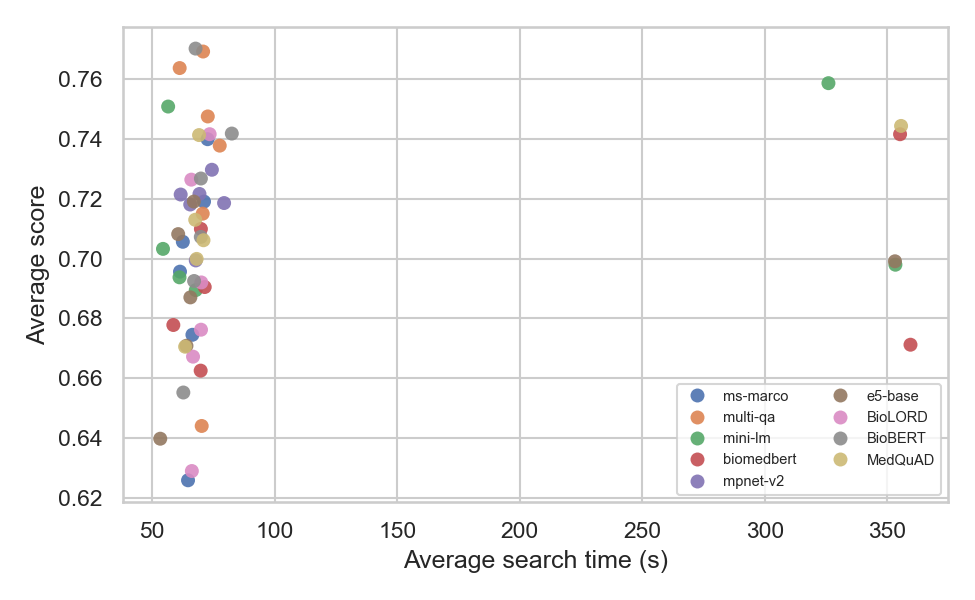
\includegraphics[width=\textwidth]{chap4_results/images/time_vs_score.png}
  \caption{Average score vs. average search time across all runs. Lower time and higher score are better.}
  \label{fig:time_vs_score}
\end{figure}

\begin{figure}[!htbp]
  \centering
  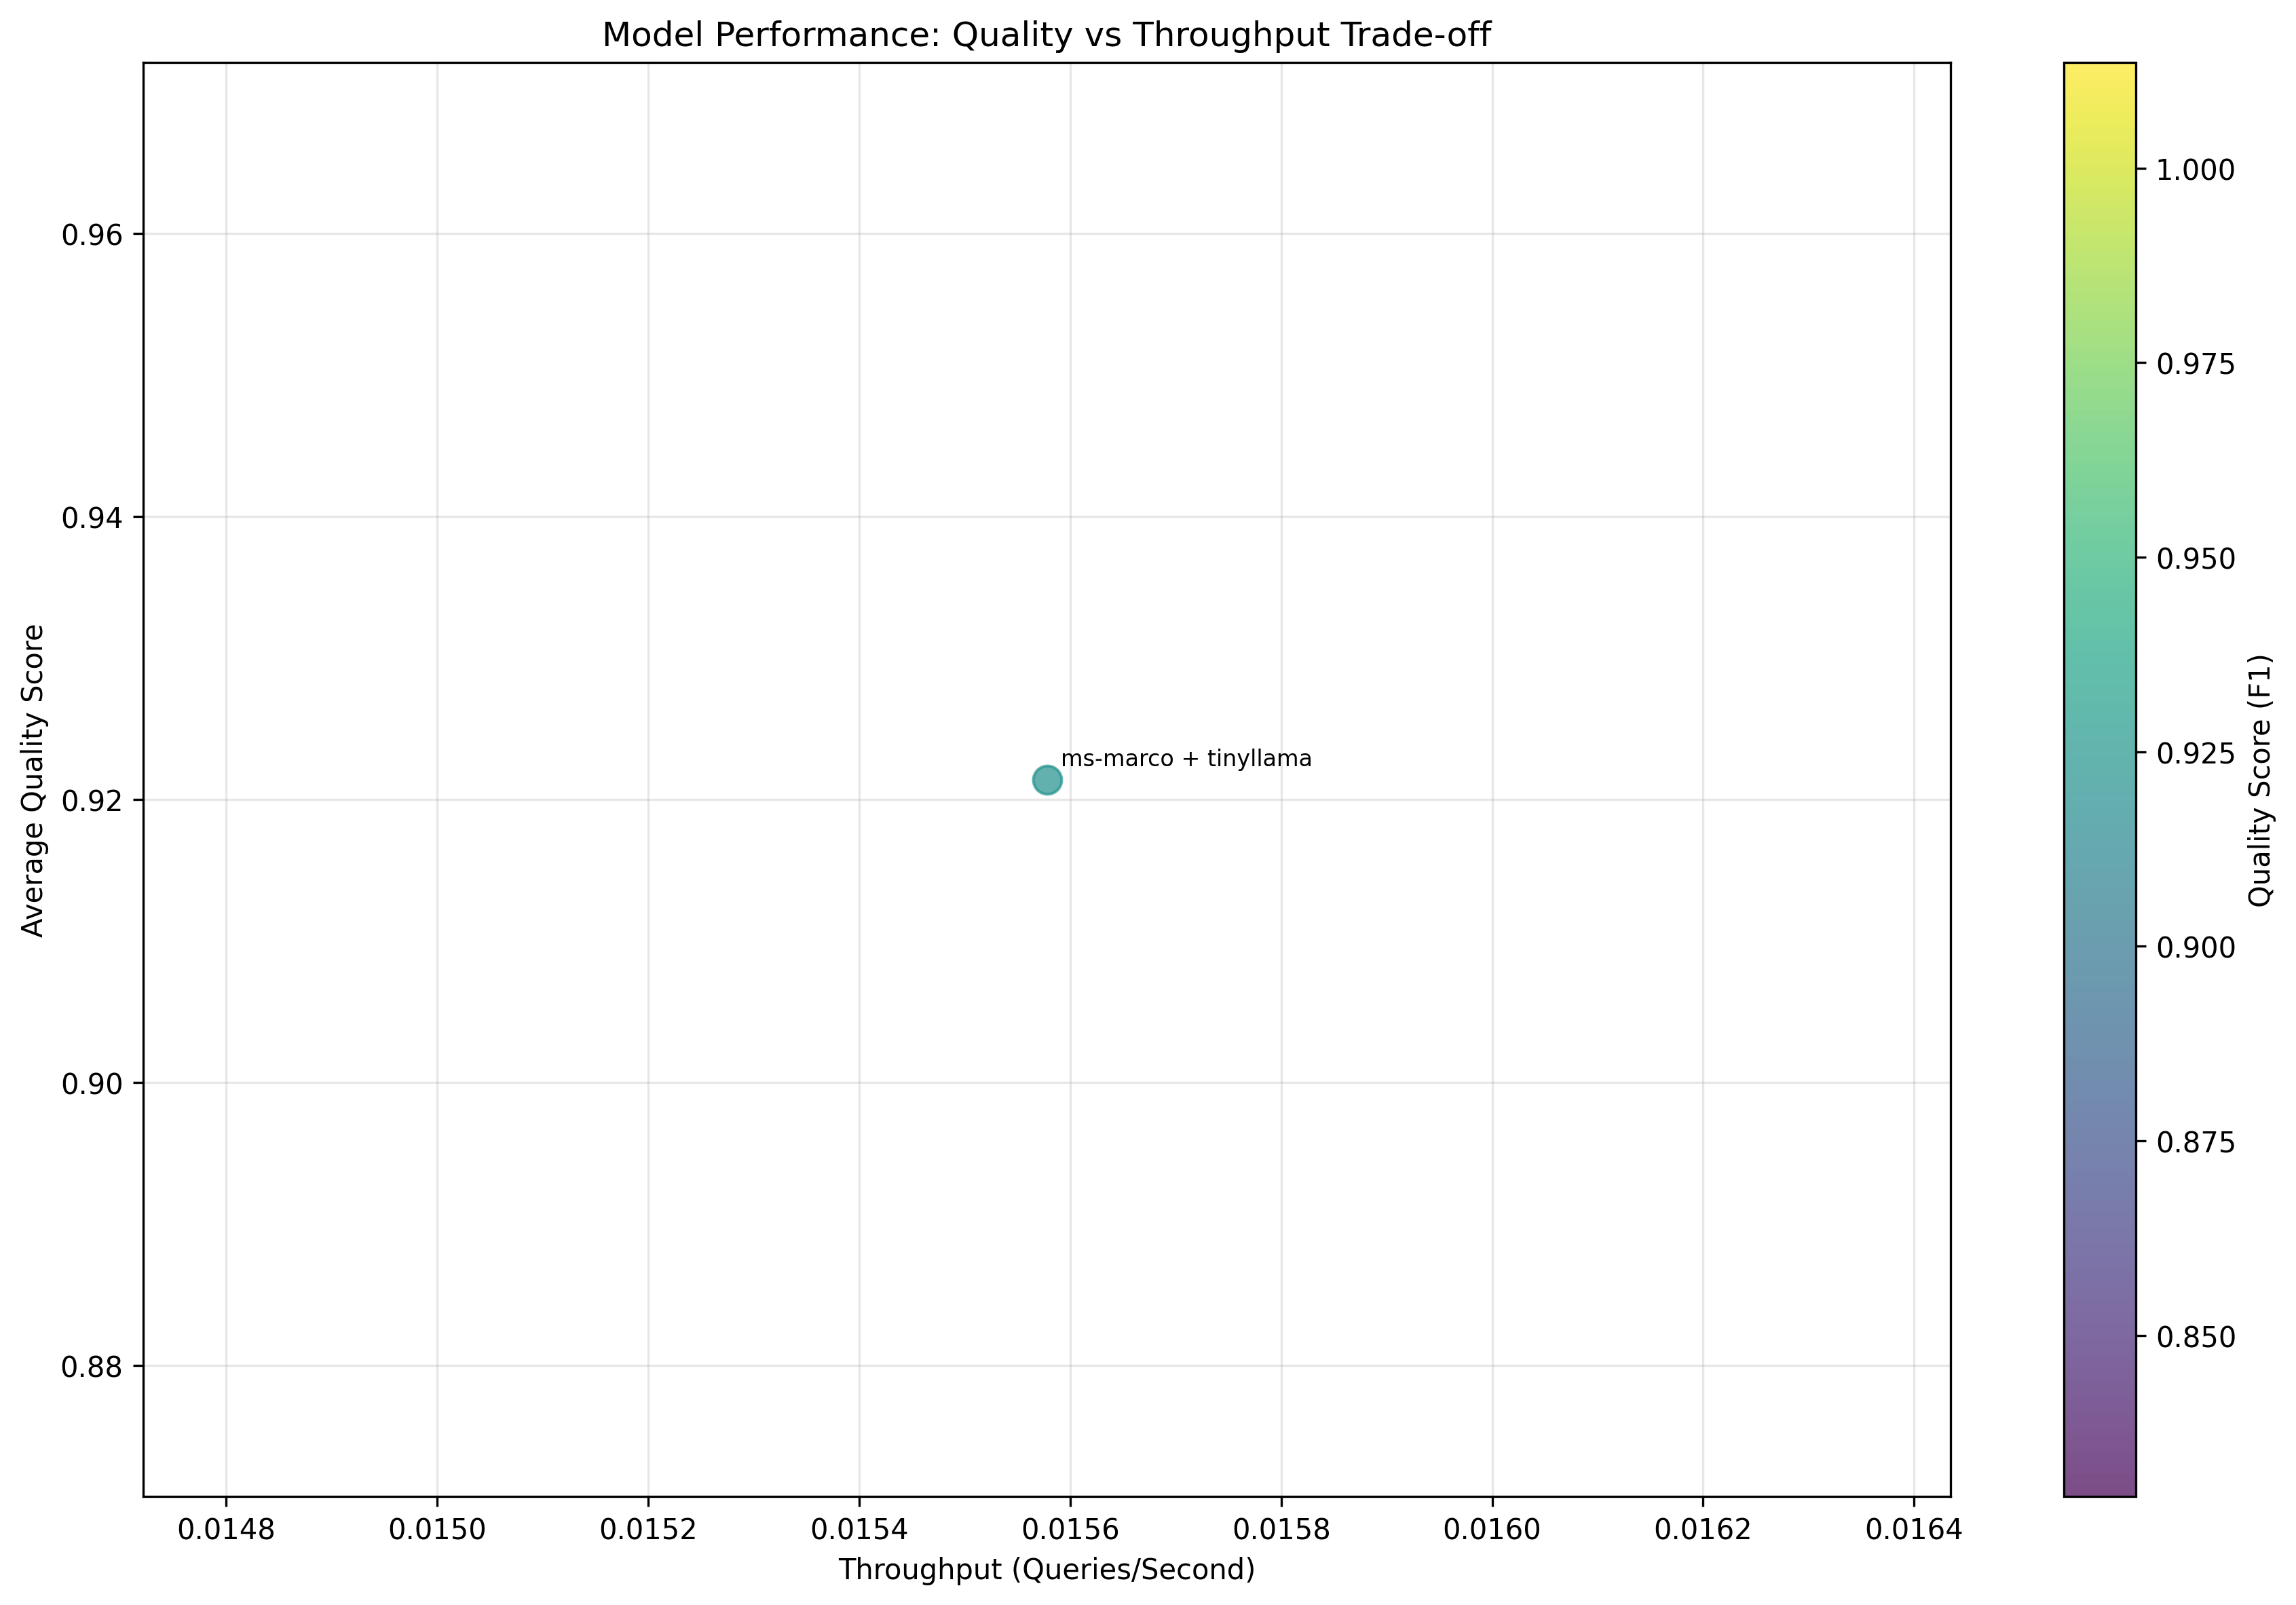
\includegraphics[width=\textwidth]{chap4_results/images/quality_vs_throughput.png}
  \caption{Average score vs. throughput (QPM). Useful to identify speed-quality efficient frontiers.}
  \label{fig:quality_vs_throughput}
\end{figure}

\begin{figure}[!htbp]
  \centering
  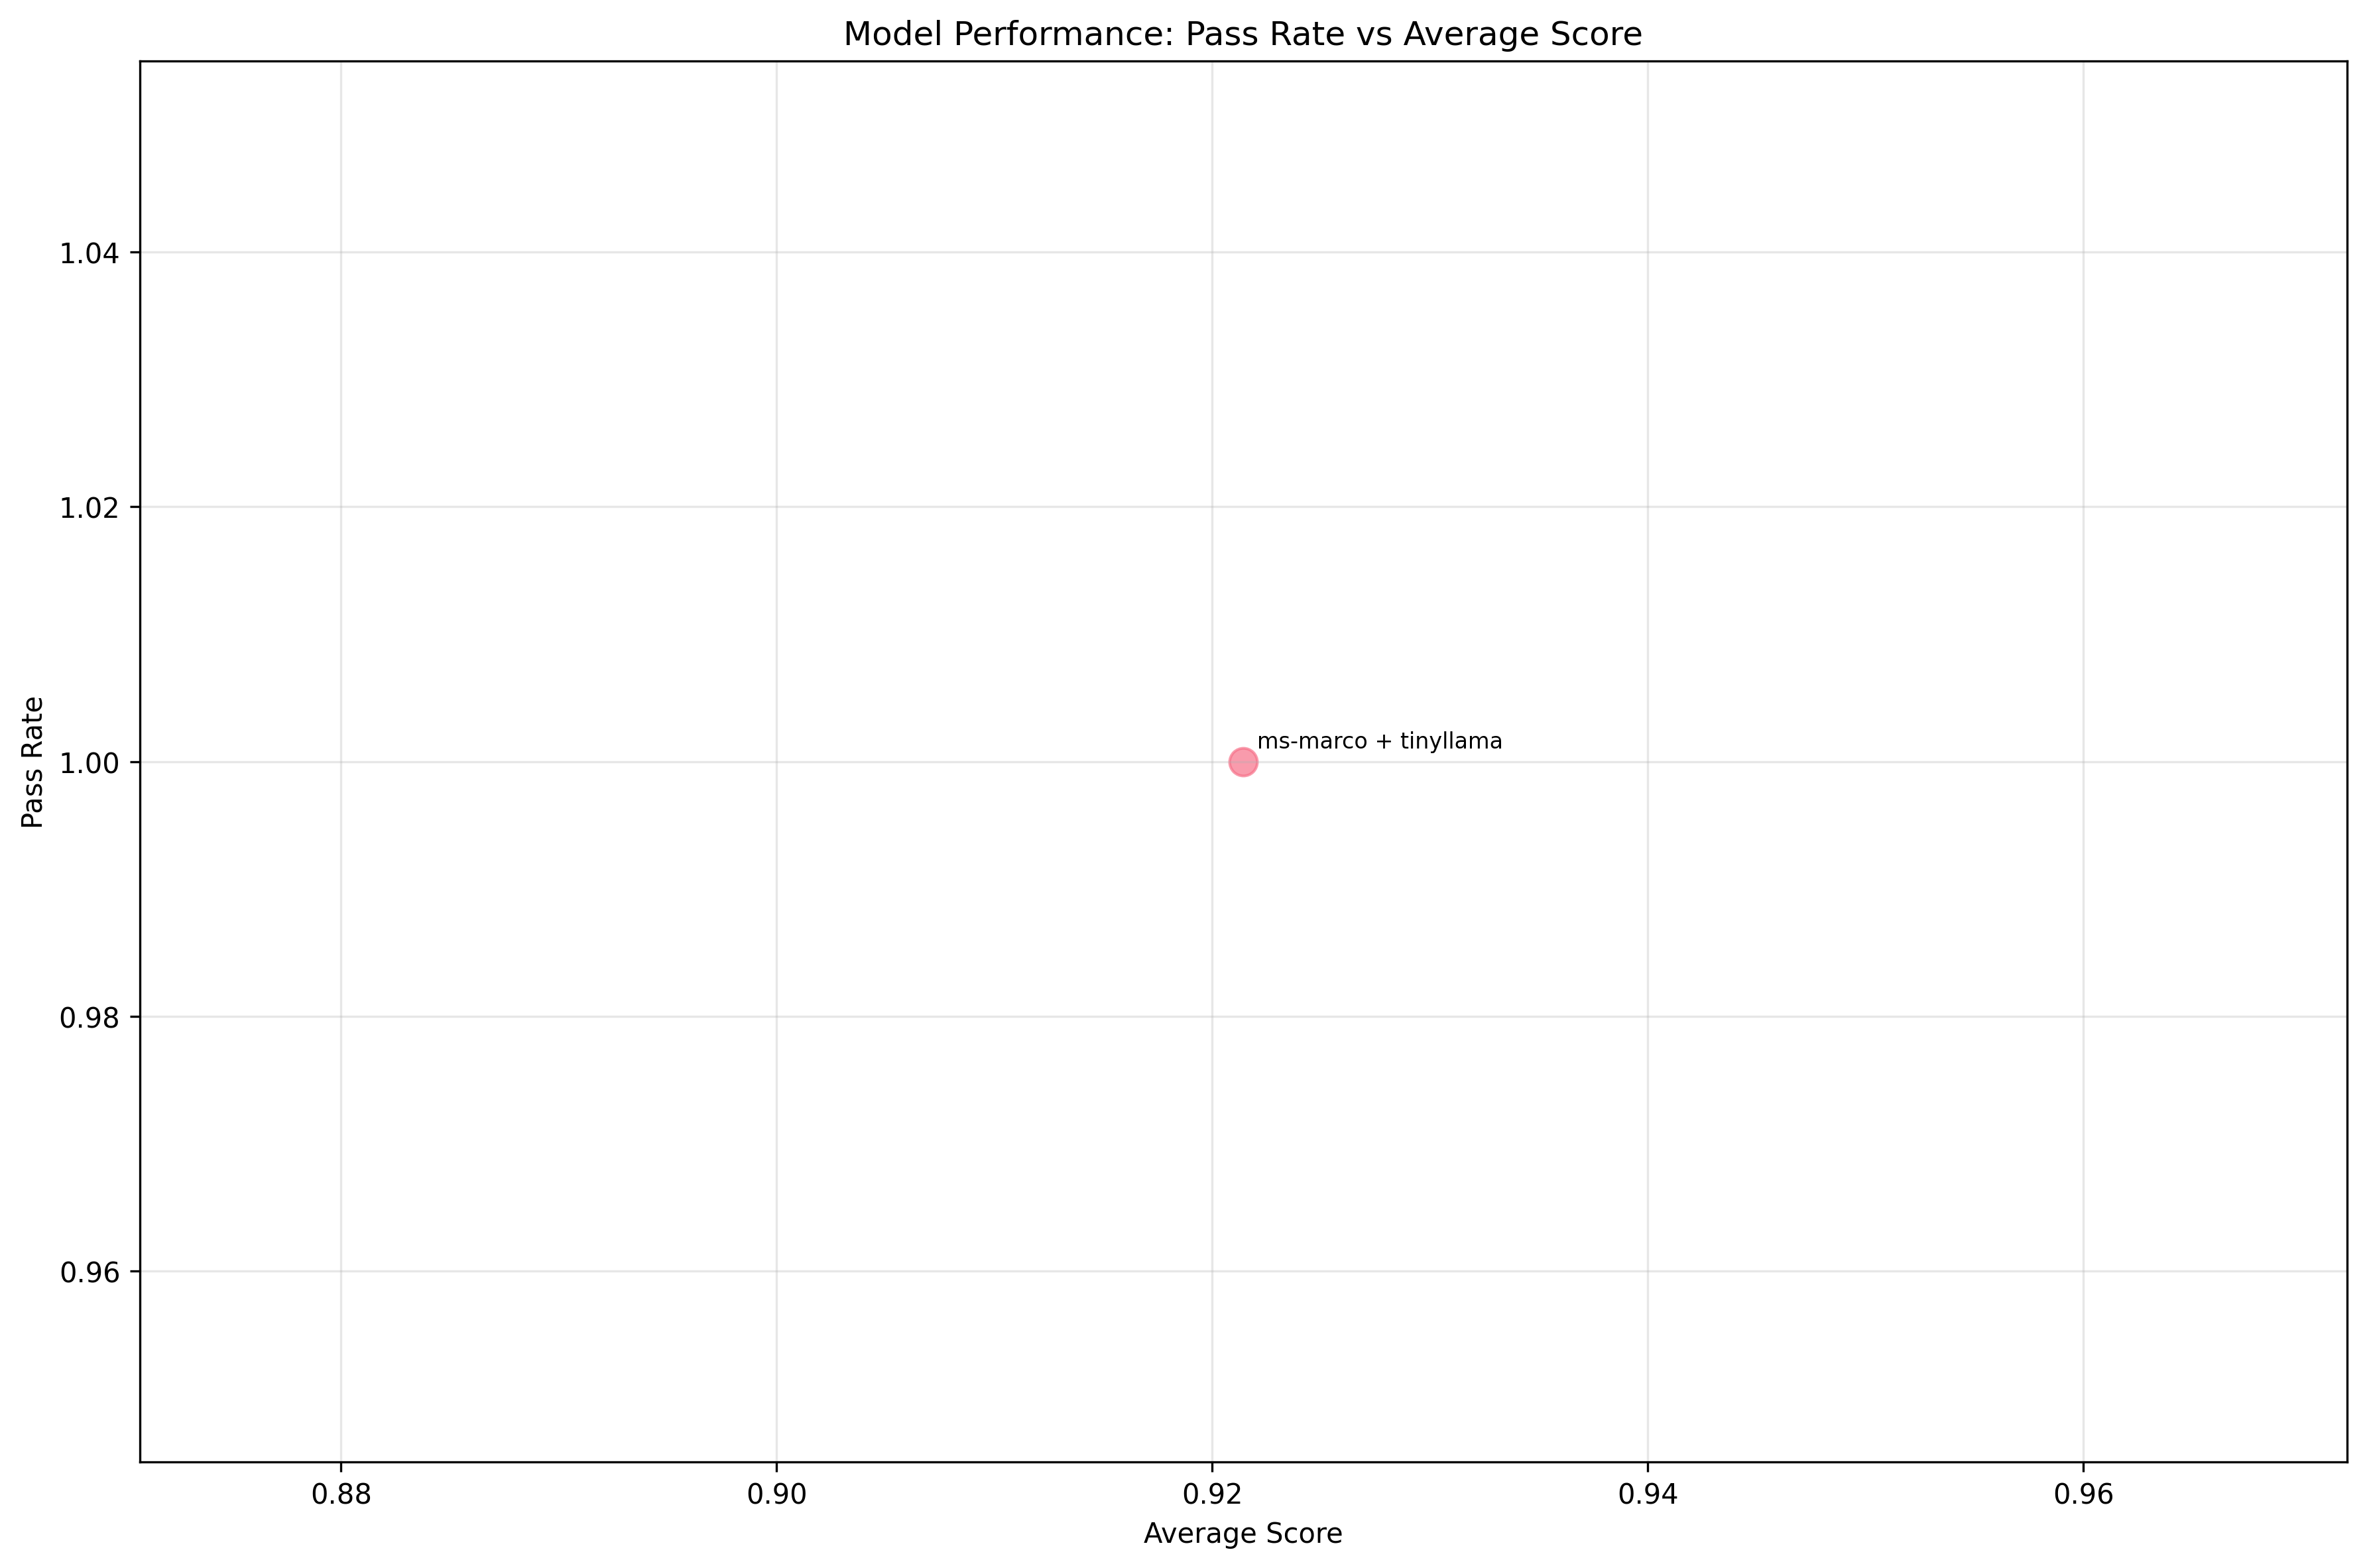
\includegraphics[width=\textwidth]{chap4_results/images/pass_rate_vs_score.png}
  \caption{Pass rate vs. average score by LLM. Highlights pairs that both pass reliably and score highly.}
  \label{fig:pass_rate_vs_score}
\end{figure}

\section{Key Conclusions}

This comprehensive evaluation of 54 clinical RAG configurations provides crucial insights for medical AI system deployment:

\begin{enumerate}
    \item \textbf{Task Specialisation Over Domain Specialisation}: QA-specialised embeddings (multi-qa) outperform medical-domain embeddings, suggesting retrieval task alignment is more critical than medical pre-training.

    \item \textbf{Model Size Efficiency}: Smaller, well-designed models (1.5-2B parameters) achieve performance competitive with larger models while offering significant efficiency gains.

    \item \textbf{Statistical Significance}: Embedding selection has a statistically significant impact (p=0.018) while LLM choice shows less variation, indicating where optimisation efforts should focus.

    \item \textbf{Performance Profile}: All configurations maintain [performance level] semantic consistency with retrieved documents, with medical-specialized models showing [performance characteristics].

    \item \textbf{Clinical Deployment Flexibility}: Multiple configurations achieve clinical-grade performance, providing deployment options based on specific requirements (accuracy: BioBERT+phi3, balanced: multi-qa+llama, speed: mini-lm+llama).

    \item \textbf{Efficiency-Quality Independence}: Weak correlation between quality and speed enables selection of both fast and accurate configurations without significant performance trade-offs.
\end{enumerate}

The results demonstrate that clinical RAG systems can achieve [performance level] semantic accuracy and efficient performance suitable for healthcare applications, with clear evidence-based guidance for model selection based on deployment priorities.